\documentclass[12pt]{article}
\usepackage{amsfonts, epsfig}

\usepackage{graphicx}
\usepackage{fancyhdr}
\pagestyle{fancy}
\lfoot{\texttt{coms30127.github.io}}
\lhead{Computation Neuroscience - 03.2\_hopfield - Conor}
\rhead{\thepage}
\cfoot{}

\usepackage{graphicx}

\usepackage{listings}

\usepackage{tikz}

\usepackage{pgf}
\usepackage[utf8]{inputenc}
\usetikzlibrary{arrows,automata}
\usetikzlibrary{positioning}


\tikzset{
    state/.style={
           rectangle,
           rounded corners,
           draw=black, very thick,
           inner sep=2pt,
           text centered,
           },
}
\tikzset{
    on/.style={
           circle,
           draw=red, very thick,
           inner sep=2pt,
           fill=red!25,
           },
}


\tikzset{
    off/.style={
           circle,
           draw=blue, very thick,
           inner sep=2pt,
           text centered,
           },
}



\tikzset{
    neuron/.style={
           rectangle,
           rounded corners,
           draw=black, very thick,
           inner sep=2pt,
           text centered,
           },
}



\tikzset{
    area/.style={
           rectangle,
           draw=black, very thick,
           inner sep=2pt,
           text centered,
           },
}


\tikzset{
    gc/.style={
           rectangle,
           rounded corners,
           draw=red, very thick,
           inner sep=2pt,
           text centered,
           },
}


\tikzset{
    inh/.style={
           rectangle,
           rounded corners,
           draw=blue, very thick,
           inner sep=2pt,
           text centered,
           },
}



\tikzset{
    io/.style={
           rectangle,
           draw=green, very thick,
           inner sep=2pt,
           text centered,
           },
}

\usepackage{ifthen}
\newboolean{nopics}
\setboolean{nopics}{true}


\begin{document}

\subsection*{Hopfield network}

A Hopfield network is a recurrently connected network; it is intended
to perform pattern completion and was proposed by John Hopfield in
1982 \cite{Hopfield1982}, though other people had had the idea before
in different contexts. The idea behind a Hopfield network is that you
evolve the network according to the McCulloch-Pitts relation, so, in
the synchronous update version, from one iteration to the next
\begin{equation}
\hat{x}_i=\phi\left(\sum_j w_{ij} x_j\right)
\end{equation}
and then $x_i\rightarrow \hat{x}$; that is all the nodes update using
the old values. In the most common version of a Hopfield network, the $w_{ij}$ are symmetric, that is
\begin{equation}
w_{ij}=w_{ji}
\end{equation}
The threshold values $\theta_i$ have been set to zero, this is
something you can do in a Hopfield network if you want because the
learning rule doesn't change to threshold. In the asynchronous scheme,
the you update the nodes one-by-one, for example, after choosing a
random node; for simplicity we stick to synchronous updates here.

The idea is that this is a model for \textsl{auto-associative}
memory. Auto-associative memories are patterns representing memories
along with some dynamics that complete partial patters. Imagine a
sequence of McCulloch-Pitts neurons
%
\ifthenelse{\boolean{nopics}}
             {\begin{quote}\textsl{There are nine circles in a row, from the left cicles one, three and six are red, the rest are blue.}\end{quote}}
             {
               \begin{center}
  
\begin{tikzpicture}
\filldraw[color=red!60, fill=red!25, very thick](0,0) circle (.25);
\filldraw[color=blue!60, fill=red!0, very thick](1,0) circle (.25);
\filldraw[color=red!60, fill=red!25, very thick](2,0) circle (.25);
\filldraw[color=blue!60, fill=red!0, very thick](3,0) circle (.25);
\filldraw[color=blue!60, fill=red!0, very thick](4,0) circle (.25);
\filldraw[color=red!60, fill=red!25, very thick](5,0) circle (.25);
\filldraw[color=blue!60, fill=red!0, very thick](6,0) circle (.25);
\filldraw[color=blue!60, fill=red!0, very thick](7,0) circle (.25);
\filldraw[color=blue!60, fill=red!0, very thick](8,0) circle (.25);
\end{tikzpicture}
               \end{center}
}
%
where the filled circles correspond to on. Recall occurs when the network is presented with a partial pattern and evolves into the complete patterns.
%
\ifthenelse{\boolean{nopics}}
           {\begin{quote}\textsl{There are two rows of nine circles, one above the other, in the top row circles one and six are red, the rest blue; in the lower row three is also red; there is an arrow from the top row to the bottom one.}\end{quote}}
             {
             \begin{center}
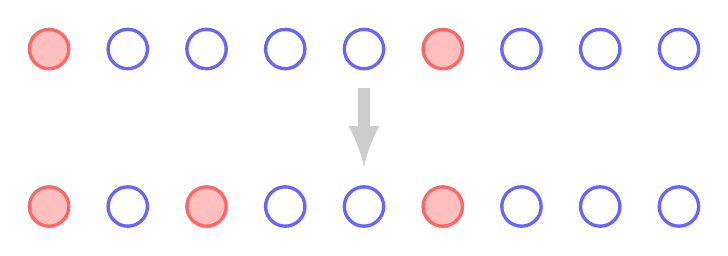
\begin{tikzpicture}
\filldraw[color=red!60, fill=red!25, very thick](0,2) circle (.25);
\filldraw[color=blue!60, fill=red!0, very thick](1,2) circle (.25);
\filldraw[color=blue!60, fill=red!0, very thick](2,2) circle (.25);
\filldraw[color=blue!60, fill=red!0, very thick](3,2) circle (.25);
\filldraw[color=blue!60, fill=red!0, very thick](4,2) circle (.25);
\filldraw[color=red!60, fill=red!25, very thick](5,2) circle (.25);
\filldraw[color=blue!60, fill=red!0, very thick](6,2) circle (.25);
\filldraw[color=blue!60, fill=red!0, very thick](7,2) circle (.25);
\filldraw[color=blue!60, fill=red!0, very thick](8,2) circle (.25);
\coordinate (a) at (4,1.5);
\coordinate (b) at (4,0.5);
\draw[->, >=latex, black!20!white, line width=4pt]   (a) to (b) ;
\filldraw[color=red!60, fill=red!25, very thick](0,0) circle (.25);
\filldraw[color=blue!60, fill=red!0, very thick](1,0) circle (.25);
\filldraw[color=red!60, fill=red!25, very thick](2,0) circle (.25);
\filldraw[color=blue!60, fill=red!0, very thick](3,0) circle (.25);
\filldraw[color=blue!60, fill=red!0, very thick](4,0) circle (.25);
\filldraw[color=red!60, fill=red!25, very thick](5,0) circle (.25);
\filldraw[color=blue!60, fill=red!0, very thick](6,0) circle (.25);
\filldraw[color=blue!60, fill=red!0, very thick](7,0) circle (.25);
\filldraw[color=blue!60, fill=red!0, very thick](8,0) circle (.25);
\end{tikzpicture}
\end{center}
}
The Hopfield network is intended to model the recall, and learning, of
memories in an autoassociative network.

One way to think about this is to note that there is an
\lq{}energy\rq{} associated with a Hopfield network:
\begin{equation}
E=-\frac{1}{2}\sum_{ij} w_{ij}x_ix_j
\end{equation}
and you can show than if you update a node you will reduce the energy.
Roughly speaking if you update a node $x_i$ then it is more likely to
have the same sign as a connected node $x_j$ if the connection between
them is large and positive since this means $w_{ij}x_j$ will have a
big effect on the activation of $x_i$ and vice versa. $x_i$ and $x_j$
are more likely to have an opposite sign if the connection is large
and negative. Thus, updating will tend to make terms like
$w_{ij}x_ix_j$ into a positive number if $w_{ij}$ is large and so that
updating the neurons will tend to reduce the energy. In fact, this can
be proved and that the system will evolve to a local minimum.

Now, if the dynamics reduces the energy, $E$, the goal is to pick the
connection strenghts so that the minima of $E$ correspond to the
patterns that the network is charged with storing. Now the question
is how to create the correct local minima? Here is a rules to achieve this:
\begin{equation}
  w_{ij}=\frac{1}{N}\sum_a x^a_ix^a_j
  \label{eq:hop}
\end{equation}
where $N$ is the number of patterns to be stored, and $a$ indexes the
patterns. There are other rules, in fact there are rules that can
store more patterns, but this rule, a sort of \lq{}top down\rq{} rule is
inspired by Hebbian plasticity. There is an online rule that is even
closer to Hebbian plasticity where $w_{ij}$ is changed for each
presentation:
\begin{equation}
\delta w_{ij}=\frac{\eta}{4} (x_i^a+1-2\alpha)(x_j^a+1-2\alpha)
\end{equation}
The idea is that following this online rule will bring you to the
values in the formula for creating the correct minima:
Eqn.~\ref{eq:hop}. The $\alpha$'s are an ofset value which allow the
network to reacha stable equilibrium since $\delta w_{ij}$ should
stopping changing, on average, if the average fraction of iterations
where $x_i$ or $x_j$ is plus one is equal to $\alpha$.

These changes in the $w_{ij}$ mimick a simple version of
\textsl{Hebbian plasticity}, a putative description of how the
synapses in the brain change in response to neuronal activity.
Synaptic plasticity usually refers to the long-term changes in synapse
strength, a long term increase in synaptic strength is called
\textsl{long term potentiation} of LTP, a decrease is called
\textsl{long term depression} or LTD. It is believed that synapses
respond to their pre- and post-synaptic activity, so that the changes
depend on the behavior of the pre- and post-synaptic neurons. It is
not known in detail what rules govern this plasticity, it seems
different neurons have different plasticity rules.

The closest thing to an overall rule was formulated by Hebb in 1949
when he said \cite{Hebb1949a}:
\begin{quote}
Let us assume that the persistence or repetition of a reverberatory
activity (or \lq{}trace\rq{}) tends to induce lasting cellular changes that
add to its stability. [$\ldots$] When an axon of cell A is near enough to excite
a cell B and repeatedly or persistently takes part in firing it, some
growth process or metabolic change takes place in one or both cells
such that A's efficiency, as one of the cells firing B, is increased.
\end{quote}
In other words, if one neurons tends to cause another to fire, the
synapse from the first to the second will get stronger. In artificial
neurons or rate-based neurons, lack spiking dynamics and instead have
a continuous state or rate variable; since \textsl{Hebbian plasticity}
often plays a role in artificial neural networks it is often applied
to a rule that strengthens synapses between neurons that are active at
the same time, that is, the explicit causal structure is ignored in
favor of
\begin{quote}
Neurons that fire together wire together.
\end{quote}
This leads to a plasticity rule 
\begin{equation}
\delta w_{ij}=\eta x_i x_j
\end{equation}
where $w_{ij}$ is the strength of the synapse from neuron $i$ to
neuron $j$, $x_i$ and $x_j$ are the states of the two neurons and
$\eta$ is a learning rate. Another version is
\begin{equation}
\delta w_{ij}=\eta (x_i-\alpha)(x_j-\alpha)
\end{equation}
where having $\alpha$ allows for different cut-off points between the behaviour that causes potentiation or depression. 

This is clearly, up to a change in variables for the $\alpha$ and
rescaling of $\eta$, this is the same as the rule
\begin{equation}
\delta w_{ij}=\frac{\eta}{4} (x_i^a+1-2\alpha)(x_j^a+1-2\alpha)
\end{equation}
mentioned for Hopfield networks; in fact, in the Hopfield network
$\alpha$ has to be set equal to the average density of the patterns,
that is, the average number of ones, for convergence.

So, to recap, during learning the patterns are activated and plastic
changes are made to the synapse strength according to a simple
correlation based Hebbian plasticity rule. In the brain, the idea is
that outside activity, signals from outside the auto-associative
network, will cause some of the neurons, the pattern to be learned, to
be active while others remain dormant. During this time plasticity
occurs. Later, during recall, the outside activity causes a fraction
of the pattern to become activity. The internal dynamics of the
network, the McCulloch-Pitts updates, cause other neurons to also
become active, allowing the pattern to repeat.

Typically $\alpha$ is very small for real networks so there will be a
large increase for the connection between two neurons that are active
at the same time, a tiny increase for pairs neurons that are inactive
at the same time and a medium size decrease for pairs of neurons where
one is active and one inactive. See Fig.~\ref{fig:hebb}.

\begin{figure}
  \ifthenelse{\boolean{nopics}}
               {{\textsl{There are nine circles in a row, from the left cicles one, three and six are red, the rest are blue. Each pair of circles is joined by a line; if both circles in the pair are red the line joining them is also red, if both circles are blue, the line is black, if one circle is red and the other blue, the line is yellow.}}}
             {
\begin{center}
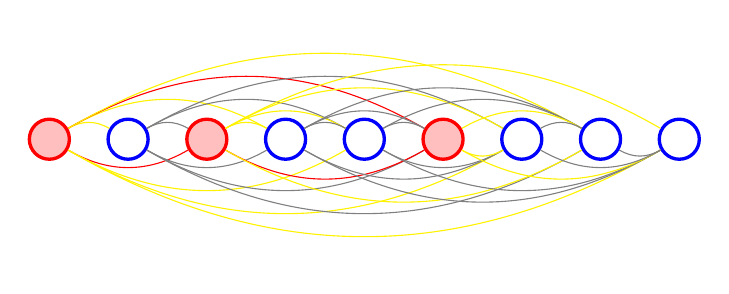
\begin{tikzpicture}
\node[on,text width=0.35cm](0){};
\node[off,text width=0.35cm,right of = 0](1){};
\node[on,text width=0.35cm,right of = 1](2){};
\node[off,text width=0.35cm,right of = 2](3){};
\node[off,text width=0.35cm,right of = 3](4){};
\node[on,text width=0.35cm,right of = 4](5){};
\node[off,text width=0.35cm,right of = 5](6){};
\node[off,text width=0.35cm,right of = 6](7){};
\node[off,text width=0.35cm,right of = 7](8){};
\path (0) edge[bend left,color=yellow] (1);
\path (0) edge[bend right,color=red] (2);
\path (0) edge[bend left,color=yellow] (3);
\path (0) edge[bend right,color=yellow] (4);
\path (0) edge[bend left,color=red] (5);
\path (0) edge[bend right,color=yellow] (6);
\path (0) edge[bend left,color=yellow] (7);
\path (0) edge[bend right,color=yellow] (8);
\path (1) edge[bend left,color=gray] (2);
\path (1) edge[bend right,color=gray] (3);
\path (1) edge[bend left,color=gray] (4);
\path (1) edge[bend right,color=gray] (5);
\path (1) edge[bend left,color=gray] (6);
\path (1) edge[bend right,color=gray] (7);
\path (2) edge[bend left,color=yellow] (3);
\path (2) edge[bend left,color=yellow] (4);
\path (2) edge[bend right,color=red] (5);
\path (2) edge[bend left,color=yellow] (6);
\path (2) edge[bend right,color=yellow] (7);
\path (2) edge[bend left,color=yellow] (8);
\path (3) edge[bend left,color=gray] (4);
\path (3) edge[bend left,color=gray] (5);
\path (3) edge[bend right,color=gray] (6);
\path (3) edge[bend left,color=gray] (7);
\path (3) edge[bend right,color=gray] (8);
\path (4) edge[bend left,color=gray] (5);
\path (4) edge[bend right,color=gray] (6);
\path (4) edge[bend left,color=gray] (7);
\path (4) edge[bend right,color=gray] (8);
\path (5) edge[bend right,color=yellow] (6);
\path (5) edge[bend left,color=yellow] (7);
\path (5) edge[bend right,color=yellow] (8);
\path (6) edge[bend left,color=gray] (7);
\path (6) edge[bend right,color=gray] (8);
\path (7) edge[bend right,color=gray] (8);
\end{tikzpicture}
\end{center}
}
\caption{Learning in the associate network. The pattern has been imposed and connection strengths are changed. The red links increase by $\eta(1-\alpha)^2$ and the gray by $\eta(-\alpha)^2$, the yellow links decrease by $\eta \alpha(1-\alpha)$.\label{fig:hebb}}
\end{figure}

As discussed, during recall some of the neurons are held in the active
state and the rest of the network evolves according to a threshold
input rule. That means each neuron has an input given by
\begin{equation}
r_i=\sum{w_{ij}x_j}
\end{equation}
and is set in the active state if $r_i>0$. The idea is that after
learning the pattern $\{0,2,5\}$
\ifthenelse{\boolean{nopics}}
  {\begin{quote}\textsl{There are nine circles in a row, from the left cicles one, three and six are red, the rest are blue. In this picture the circles are labelled by a number, but using Python conventions, so the three red circles are labelled 0, 2 and 5.}\end{quote}}
         {
\begin{center}
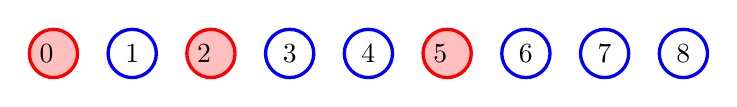
\begin{tikzpicture}
\node[on,text width=0.35cm](0){0};
\node[off,text width=0.35cm,right of = 0](1){1};
\node[on,text width=0.35cm,right of = 1](2){2};
\node[off,text width=0.35cm,right of = 2](3){3};
\node[off,text width=0.35cm,right of = 3](4){4};
\node[on,text width=0.35cm,right of = 4](5){5};
\node[off,text width=0.35cm,right of = 5](6){6};
\node[off,text width=0.35cm,right of = 6](7){7};
\node[off,text width=0.35cm,right of = 7](8){8};
\end{tikzpicture}
\end{center}
}
             the connections between these nodes will be strong, so if the network has nodes $\{0,5\}$ activated
 \ifthenelse{\boolean{nopics}}
  {\begin{quote}\textsl{There are nine circles in a row labelled zero to eight, all are blue except the cicles labelled 0 and 5.}\end{quote}}
             {
\begin{center}
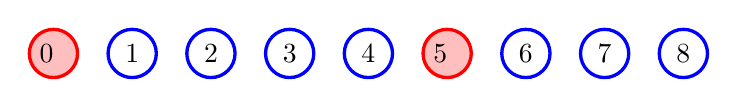
\begin{tikzpicture}
\node[on,text width=0.35cm](0){0};
\node[off,text width=0.35cm,right of = 0](1){1};
\node[off,text width=0.35cm,right of = 1](2){2};
\node[off,text width=0.35cm,right of = 2](3){3};
\node[off,text width=0.35cm,right of = 3](4){4};
\node[on,text width=0.35cm,right of = 4](5){5};
\node[off,text width=0.35cm,right of = 5](6){6};
\node[off,text width=0.35cm,right of = 6](7){7};
\node[off,text width=0.35cm,right of = 7](8){8};
\end{tikzpicture}
\end{center}
}
the value $r_{2}=w_{12}+w_{52}$ will be larger than the threshold and
the subsequent dynamics will switch neuron 2 on. However, in this
network, if a different initial set of neurons are activated, the
activity will die away because the $r_i$ will all be sub-threshold.

When many patterns are stored it is likely that there will be
interference between them. This is illustrated in
Fig.~\ref{fig:interfere}. Although the figure shows how a single
neuron fails to participate in two patterns, for larger networks some
overlap is possible, but too much overlap prevents retrieval. In fact
the capacity is proportional to the number of neurons, $N$. A
hand-waving argument goes like this: the number of connections is
roughly $N^2$ and the amount of information in a pattern is $N$ so the
number of patterns that can be stored is $N^2/N=N$ \cite{Amit1992a}.


\begin{figure}
  \ifthenelse{\boolean{nopics}}
  {{\textsl{There are two rows nine circles in a row labelled zero to eight. In the top row neurons 0, 2 and 5 are red, in the bottom, 1, 5 and 6. In each row lines connect five to the other neurons, with red lines when the other neuron is red, and yellow if the other neuron is blue.}}}
             {
\begin{center}
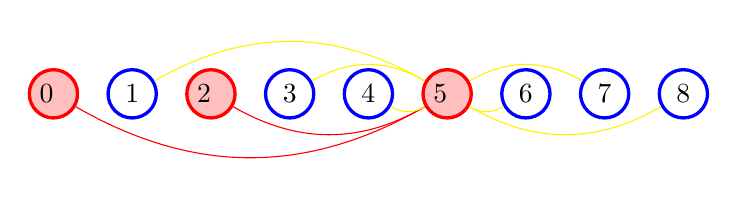
\begin{tikzpicture}
\node[on,text width=0.35cm](0){0};
\node[off,text width=0.35cm,right of = 0](1){1};
\node[on,text width=0.35cm,right of = 1](2){2};
\node[off,text width=0.35cm,right of = 2](3){3};
\node[off,text width=0.35cm,right of = 3](4){4};
\node[on,text width=0.35cm,right of = 4](5){5};
\node[off,text width=0.35cm,right of = 5](6){6};
\node[off,text width=0.35cm,right of = 6](7){7};
\node[off,text width=0.35cm,right of = 7](8){8};
\path (5) edge[bend left,color=red] (0);
\path (5) edge[bend right,color=yellow] (1);
\path (5) edge[bend left,color=red] (2);
\path (5) edge[bend right,color=yellow] (3);
\path (5) edge[bend left,color=yellow] (4);
\path (5) edge[bend right,color=yellow] (6);
\path (5) edge[bend left,color=yellow] (7);
\path (5) edge[bend right,color=yellow] (8);
\end{tikzpicture}
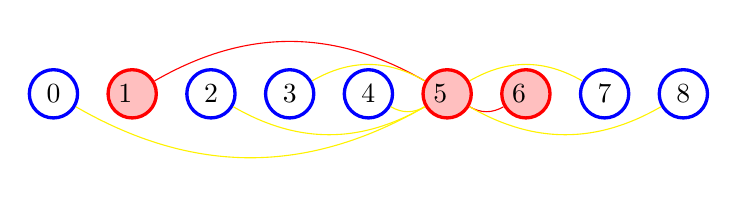
\begin{tikzpicture}
\node[off,text width=0.35cm](0){0};
\node[on,text width=0.35cm,right of = 0](1){1};
\node[off,text width=0.35cm,right of = 1](2){2};
\node[off,text width=0.35cm,right of = 2](3){3};
\node[off,text width=0.35cm,right of = 3](4){4};
\node[on,text width=0.35cm,right of = 4](5){5};
\node[on,text width=0.35cm,right of = 5](6){6};
\node[off,text width=0.35cm,right of = 6](7){7};
\node[off,text width=0.35cm,right of = 7](8){8};
\path (5) edge[bend left,color=yellow] (0);
\path (5) edge[bend right,color=red] (1);
\path (5) edge[bend left,color=yellow] (2);
\path (5) edge[bend right,color=yellow] (3);
\path (5) edge[bend left,color=yellow] (4);
\path (5) edge[bend right,color=red] (6);
\path (5) edge[bend left,color=yellow] (7);
\path (5) edge[bend right,color=yellow] (8);
\end{tikzpicture}
\end{center}
}
\caption{Interference in an auto-associative network. Neuron 5 is involved in two patterns and, as a consequence, some of its connections are strengthen for one pattern and weakened for the other, if these strengthening and weakening effects are similar in size it makes it unlikely that either pattern will be accurately retrieved.\label{fig:interfere}}
\end{figure}


The capacity is also larger if there is sparseness; one way to think
of this is to observe the weight decrease between an active and
inactive connection is $\delta w_{ij}=-\eta \alpha (1-\alpha)$ so the
smaller $\alpha$ is the smaller the amount these links are
decreased. Links are decreased if, in the pattern, one neuron is
active and one inactive, they are strengthened if both neurons are
active, the increase is $\eta (1-\alpha)^2$. Hence, it takes of the
order of $1/\alpha$ patterns where a connection is weakened to wipe
out the strengthening that results if the connection is part of a
pattern. In fact, it is estimated that the capacity of a network is
\begin{equation}
P=\frac{k}{\alpha}N
\end{equation}
where $k$ is constant which has been found to be about $k\approx
0.035$, this is reduced to 
\begin{equation}
P=c\frac{k}{\alpha}N
\end{equation}
if there are missing connections, where $c$ stands for the fraction of pairs that are connected.

The actual sparseness of the brain needs to balance this advantage,
the increased capacity, along with a metabolic advantage and more
abstract computational advantage which says that a sparse coding for
information involves object recognition or segmentation against the
disadvantages, most obviously the vulnerability of the pattern to the
loss of neurons or connections and, perhaps more importantly, a sparse
code involves fewer elements and so may be less useful for
retrieval. It is hard to actually estimate sparseness in practice
since neurons are not, in reality, on-off units.

\begin{thebibliography}{10}

\bibitem{Hopfield1982}
Hopfield, JJ. (1982) Neural networks and physical systems with emergent collective computational abilities.
\newblock Proceedings of the National Academy of Sciences of the USA, 79:2554--2558.

\bibitem{Hebb1949a}
Hebb DO. (1949) The Organization of Behavior. 
\newblock New York: Wiley \& Sons.


\bibitem{Amit1992a} Amit D. (1992) Modeling Brain Function: The World
  of Attractor Neural Networks.
\newblock Cambridge University Press, Cambridge England.


\end{thebibliography}

\end{document}

